\documentclass[12pt]{extarticle}
\usepackage[utf8]{inputenc}
\usepackage{amsmath}
\usepackage{graphicx}

\title{MATH 377: Dynamical Systems Project}
\author{Connor Gephart}
\date{14 October 2019}

\begin{document}

\maketitle
\section{Introduction}
This project began with a simple population modeling exercise. If there was a population of a type of creature that had a maximum lifespan of 3 years, how would their population change over time given birth and death rates for each age group: 0-1, 1-2, 2-3. This question was then expanded to consider a population of "Luvmee". The Luvmee species does not live past the age of 6, and is again broken up into one year age groups. The starting populations of these age groups in millions were given as the following vector $p_0$, where each entry represents an age group:
\[p_0 = \begin{bmatrix}
40\\45\\30\\50\\30\\5\\
\end{bmatrix}\]
\newline
The fertility-mortality matrix for this population is given by $M$:
\[M = \begin{bmatrix}
0&0.07&0.8&0.2&0&0\\
0.98&0&0&0&0&0\\
0&0.96&0&0&0&0\\
0&0&0.95&0&0&0\\
0&0&0&0.92&0&0\\
0&0&0&0&0.60&0\\
\end{bmatrix}\]

With the initial population and this fertility-mortality matrix, the population can be determined by computing $M^n\cdot p_0$ where $n$ is the number of years since the initial population measurement was taken. 
\section{Tasks}
\subsection{Task 1}
The first part of this project was to determine all of the eigenvalues and eigenvectors of the fertility-mortality matrix. The modulus and argument of the eigenvalues will help determine which eigenvalue controls the eventual behavior of the population, i.e. will the population stabilize, grow, or die off, and then the other eigenvalues will dictate how the population changes over time. 

All values were calculated using Mathematica. The eigenvalues, and their associated modulus and argument, if applicable, are as follows.  
\newline
$\lambda_1 = 0.999997$\\
$modulus = 0.999997$
\newline
\newline
$\lambda_2 = -0.380804 + 0.777704i$\\
$modulus = 0.865931$\\
$argument = 2.02613$
\newline
\newline
$\lambda_3 = -0.380804 - 0.777704i$\\
$modulus = 0.865931$\\
$argument = -2.02613$
\newline
\newline
$\lambda_4 = -0.238389$\\
$modulus = 0.238389$
\newline
There are two real eigenvalues, $\lambda_1$ and $\lambda_4$ and two complex eigenvalues, $\lambda_2$ and $\lambda_3$. The eigenvalue with the largest modulus is $\lambda_1$. This will be discussed later on. 
\newline
The eigenvectors corresponding to these eigenvalues are as follows.
\newline
\[e_1 = \begin{bmatrix}
 0.468094\\
 -0.0830352 + 0.324457i\\
 -0.0830352 - 0.324457i\\
 0.00144321\\
 0\\
 0
\end{bmatrix}\]
\[e_2 = \begin{bmatrix}
 0.458734\\
 0.371112 - 0.0770812i\\
 0.371112 + 0.0770812i\\
 -0.00593295\\
 0\\
 0
\end{bmatrix}\]
\[e_3 = \begin{bmatrix}
 0.440385
 -0.257679 - 0.331928i\\
 -0.257679 + 0.331928i\\
 0.0238922\\
 0\\
 0
\end{bmatrix}\]
\[e_4 = \begin{bmatrix}
 0.418367\\
 -0.202733 + 0.414034i\\
 -0.202733 - 0.414034i\\
 -0.0952125
 0\\
 0
\end{bmatrix}\]
\[e_5 = \begin{bmatrix}
 0.384899\\
 0.489789\\
 0.489789\\
 0.367448\\
 0\\
 0
\end{bmatrix}\]
\[e_6 = \begin{bmatrix}
 0.23094\\
 -0.149244 - 0.304796i\\
 -0.149244 + 0.304796i\\
 -0.924829\\
 1\\
 0
\end{bmatrix}\]

\subsection{Task 2}
The second task was to compute the population, based on $p_0$, after 30 years. The easiest way to show this was using the output from the Mathematica code, as well as two graphs created in Microsoft Excel. The Mathematica code is included mostly as a reference for the graphed data. 

First is the Mathematica results in matrix form starting at year 1, where $p_0$ is the population in year 0:
\begin{figure}[ht!]
  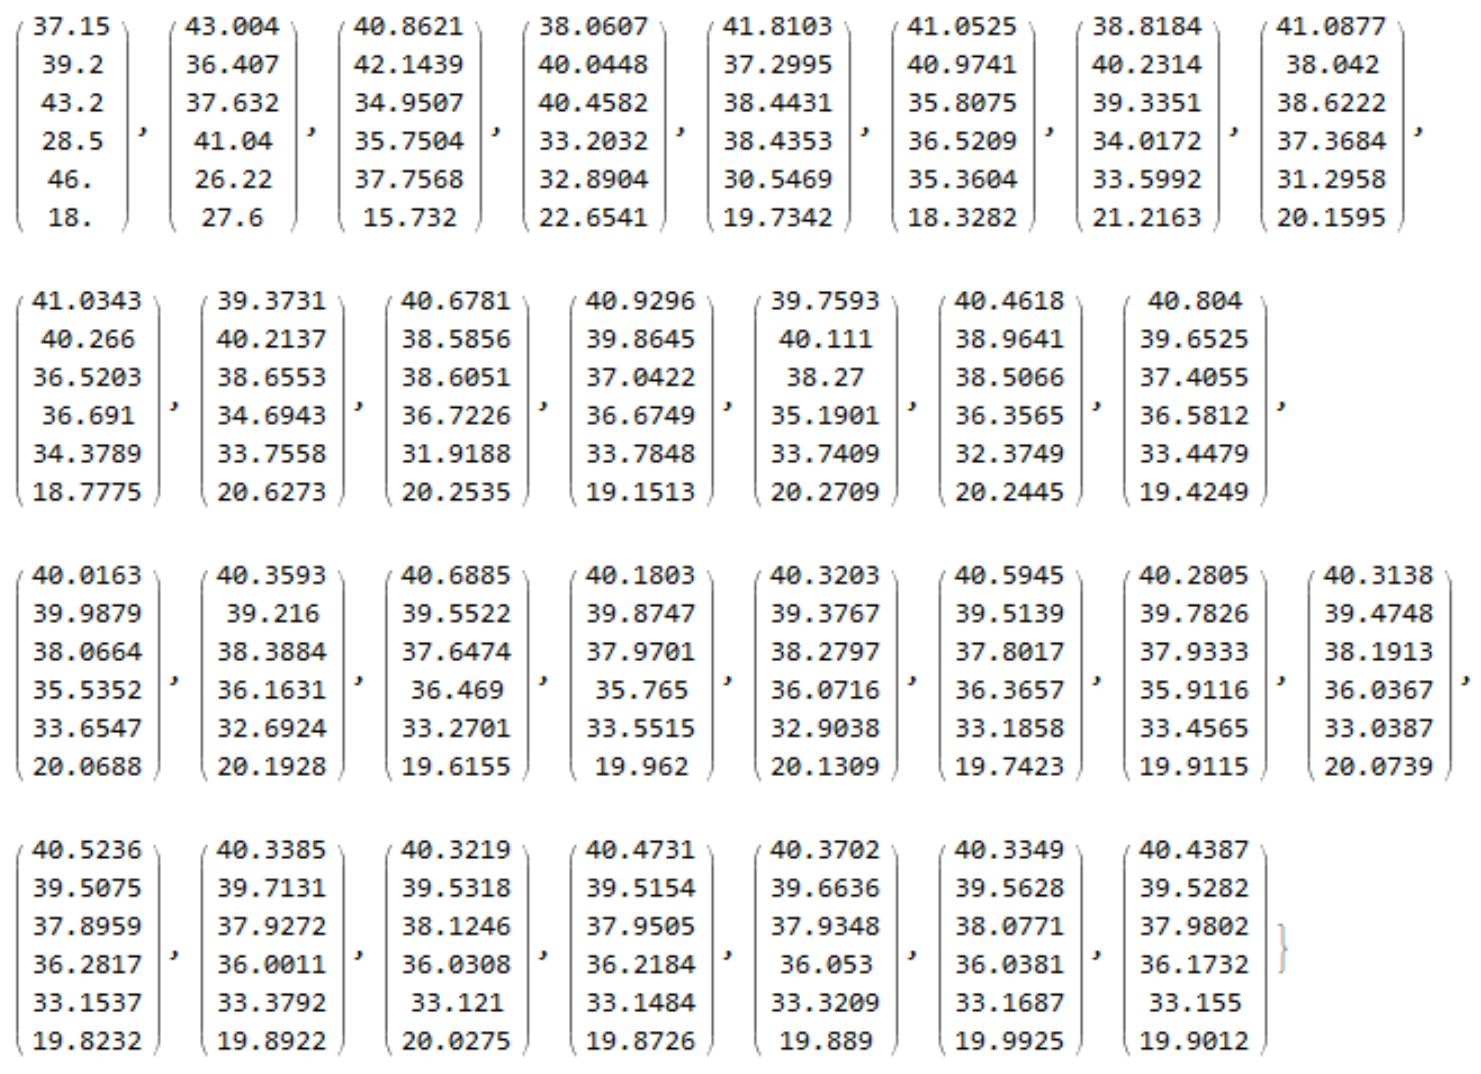
\includegraphics[width=\linewidth]{PopulationAfter30YearsMatrices.JPG}
  \caption{The population of each age group over 30 years}
\end{figure}
\newpage
\begin{figure}[ht!]
  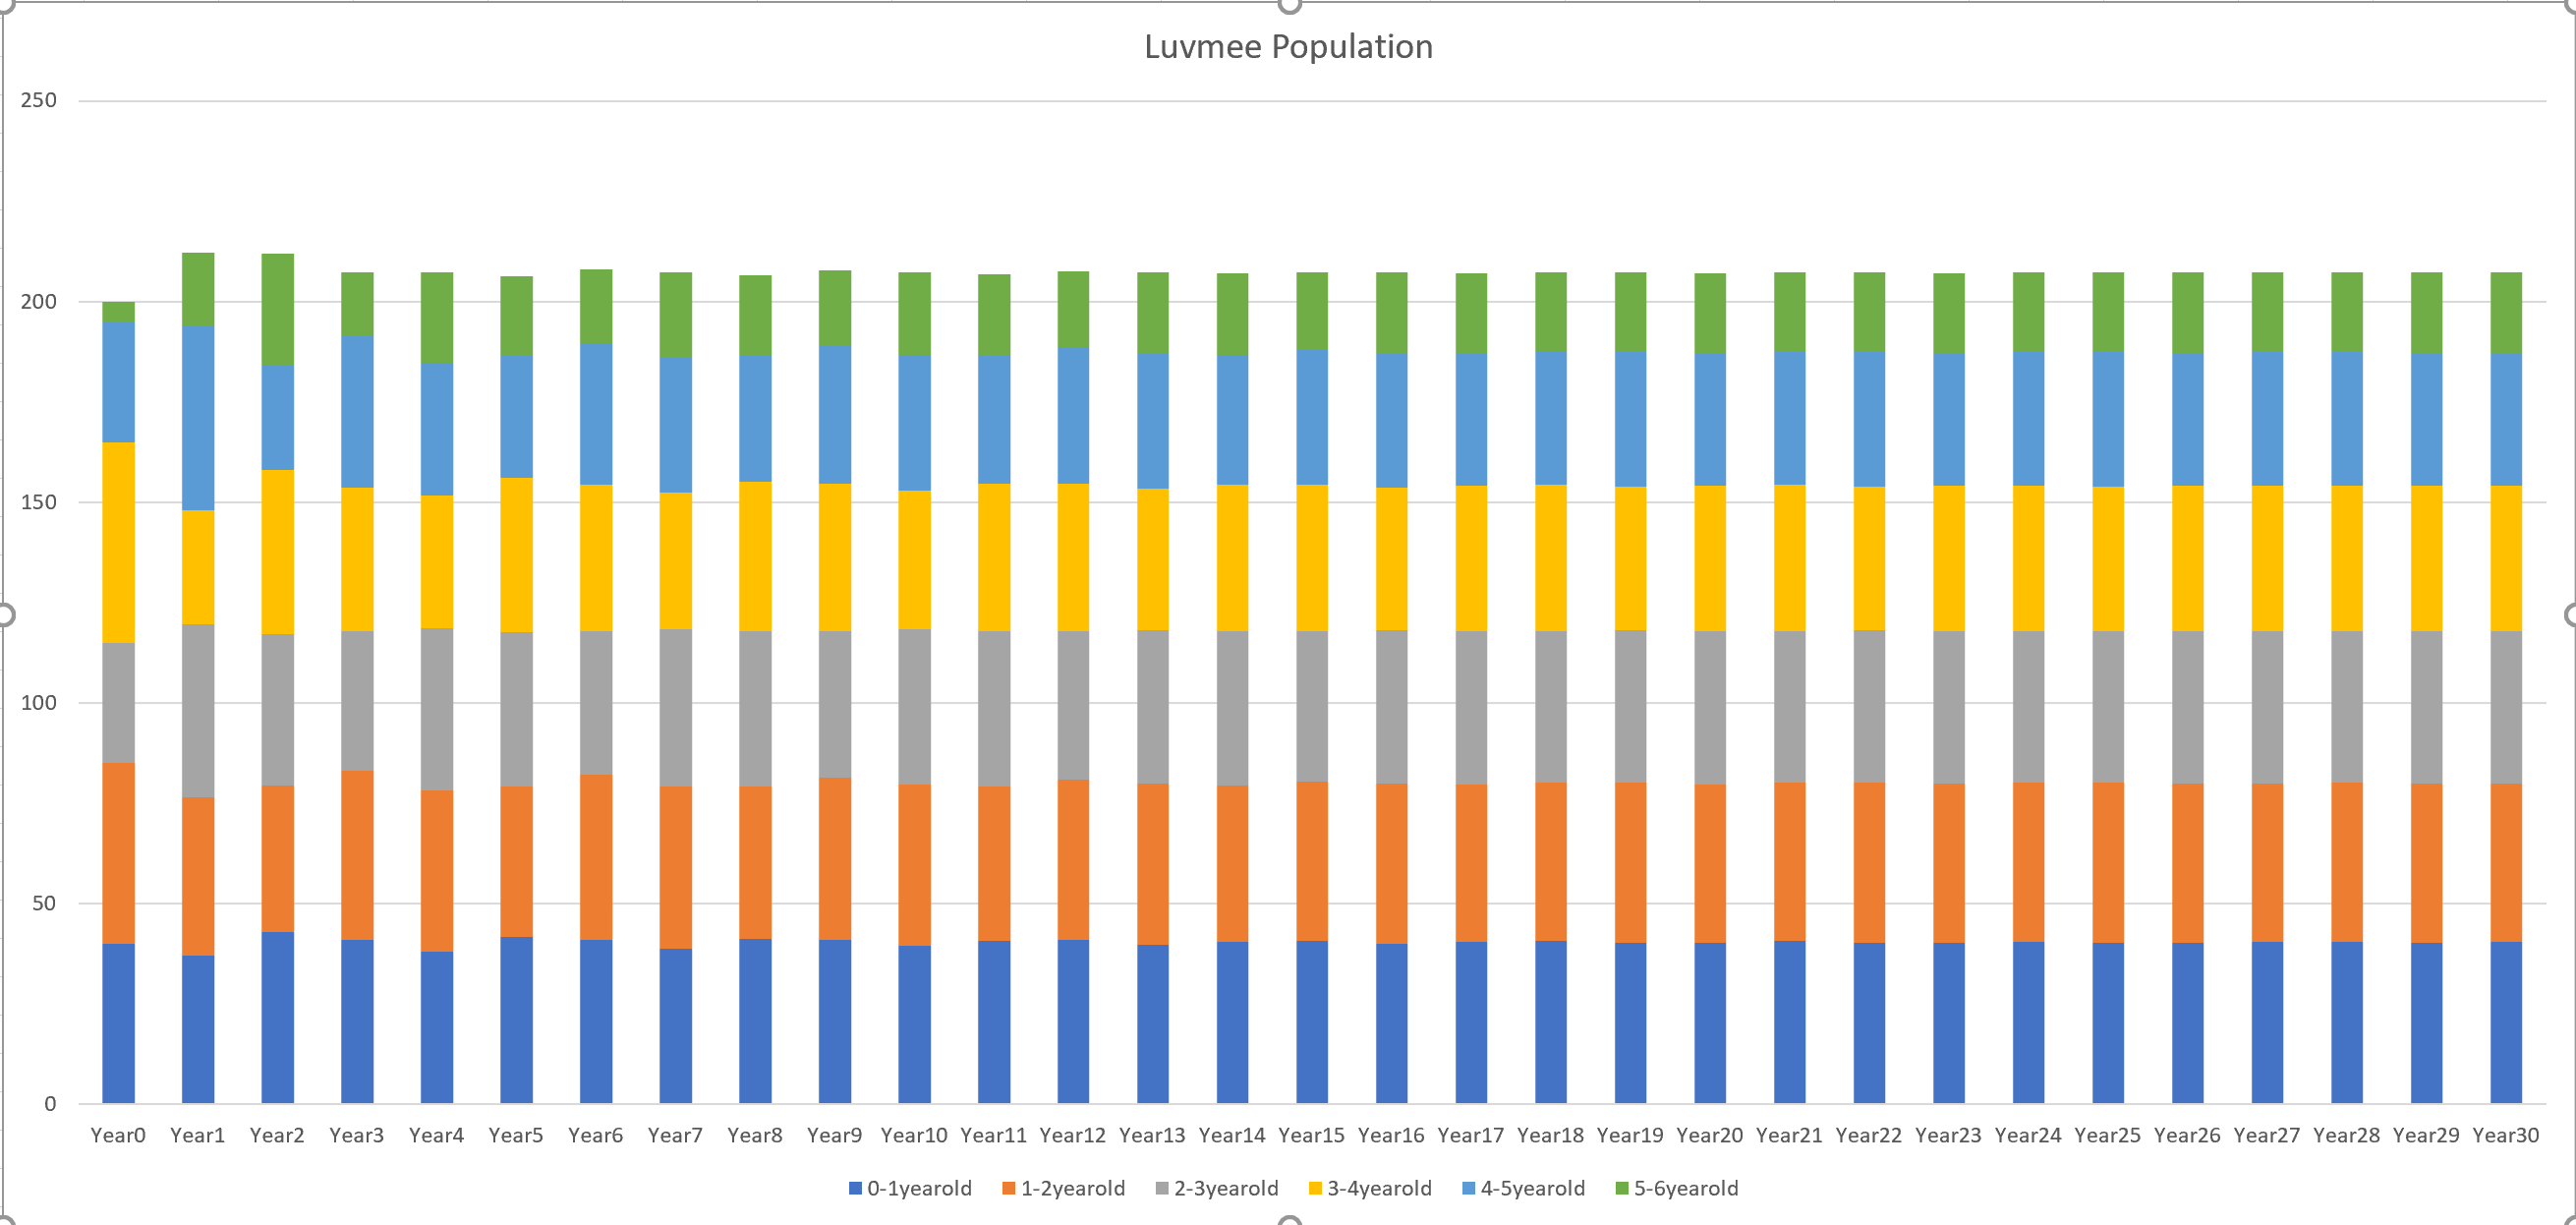
\includegraphics[width=\linewidth]{PopulationGraph2.PNG}
  \caption{Stacked bar graph of population. It can be seen from this bar graph that there is a baby boom at first, but then the population quickly stabilizes over time, with a consistent total number and proportion of each age group by the 30th year. }
\end{figure}
\newpage
\begin{figure}[ht!]
  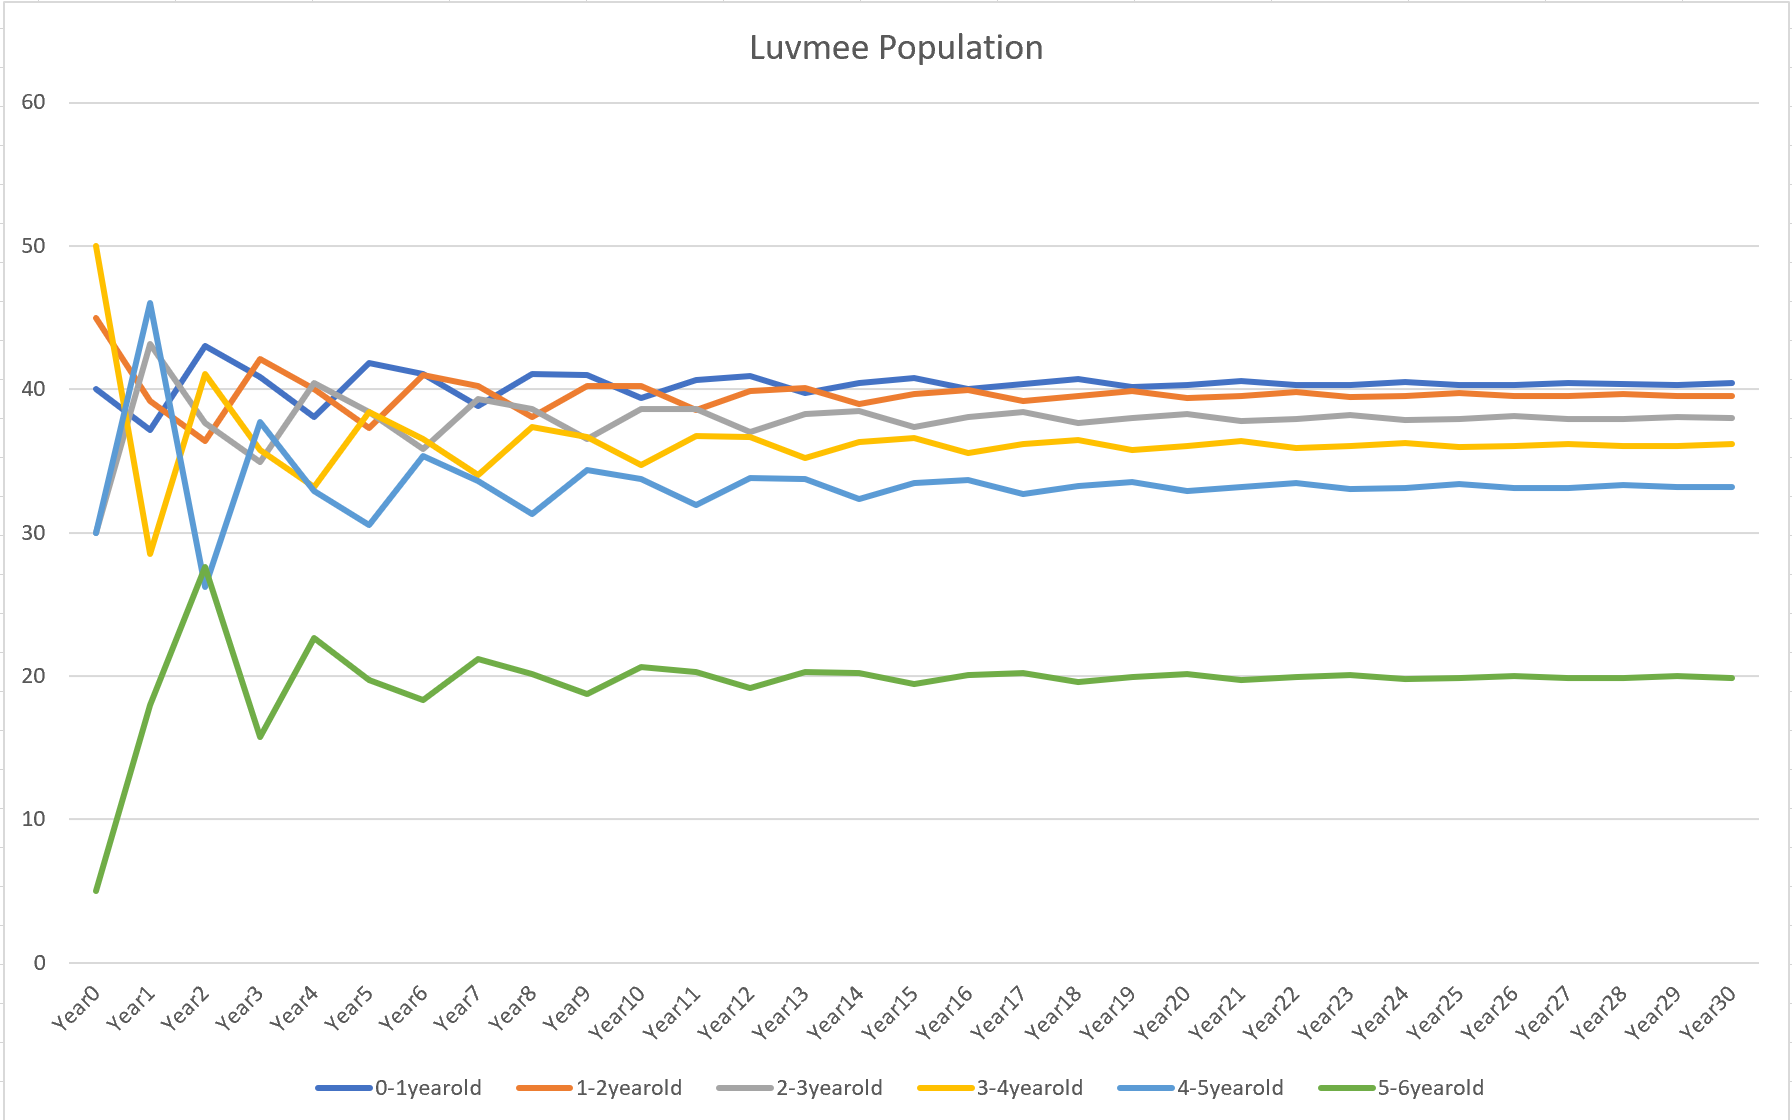
\includegraphics[width=\linewidth]{PopulationGraph1.PNG}
  \caption{Line graph of population. The line graph demonstrates the cycle of growth for each age group. While not synchronized, they all seem to follow the same 3 year cycle. }
\end{figure}
\newpage
\subsection{Task 3}
The third task was to analyze the eigenvalues and eigenvectors, and determine what the practical meaning of the eigenvector that corresponds to the eigenvalue with the largest modulus. The eigenvalue with the largest modulus is $lambda_1$ with a modulus of 0.999997 and it dictates the eventual behavior of the Luvmee population. 0.999997 can be rounded to 1, which means that this population will eventually stabilize in both size and proportions of each of the age groups. This is seen above in the graphs. If the eigenvalue were to have a modulus less than one, the population would eventually die out, and if the eigenvalue were to have a modulus greater than one, it would grow forever while eventually settling into set proportions of age groups. 
\newline
The first eigenvector can then be normalized to get the population proportion in terms of percentages. This is done by taking the eigenvector corresponding to $\lambda_1$, $e_1$ and dividing it by its 1-Norm. This yields the following vector:

\[\frac{e_1}{Norm(e_1)} = \begin{bmatrix}
0.1949\\0.1910\\0.1834\\0.1742\\0.1603\\0.0962\\
\end{bmatrix}\]
\newline
This means that 19.49\% of the population will be 0-1 year olds, 19.10\% will be 1-2, 18.34\% will be 2-3, 17.42\% will be 3-4, 16.03\% will be 4-5, and finally 9.62\% will be 5-6. 

\subsection{Task 4}
The final task was to describe the behavior of the remaining eigenvectors in the context of a new starting point:
\[p_0 = \begin{bmatrix}
29.0265\\26.0768\\60.9976\\26.1274\\11.8528\\37.9621
\end{bmatrix}\]

This initial population was chosen to emphasize the cycle of baby booms and baby busts. This can be seen by looking at the first 30 years of population dynamics shown below. At first, the size of each population varies significantly from year to year, but as time goes on, the effects of the other eigenvetors begin to shrink, allowing the population to stabilize. The cycle seems to be about 3 years in length, with a baby boom the first year, and then declining the second and third years. This trend holds until approximately the 16th year, at which point the population has already mostly stabilized. The trend is felt in the older age ranges, each offset by one year. For example, a baby boom occurs the first year, so the population of 1-2 year olds is larger in the second year. 

\begin{figure}[ht!]
  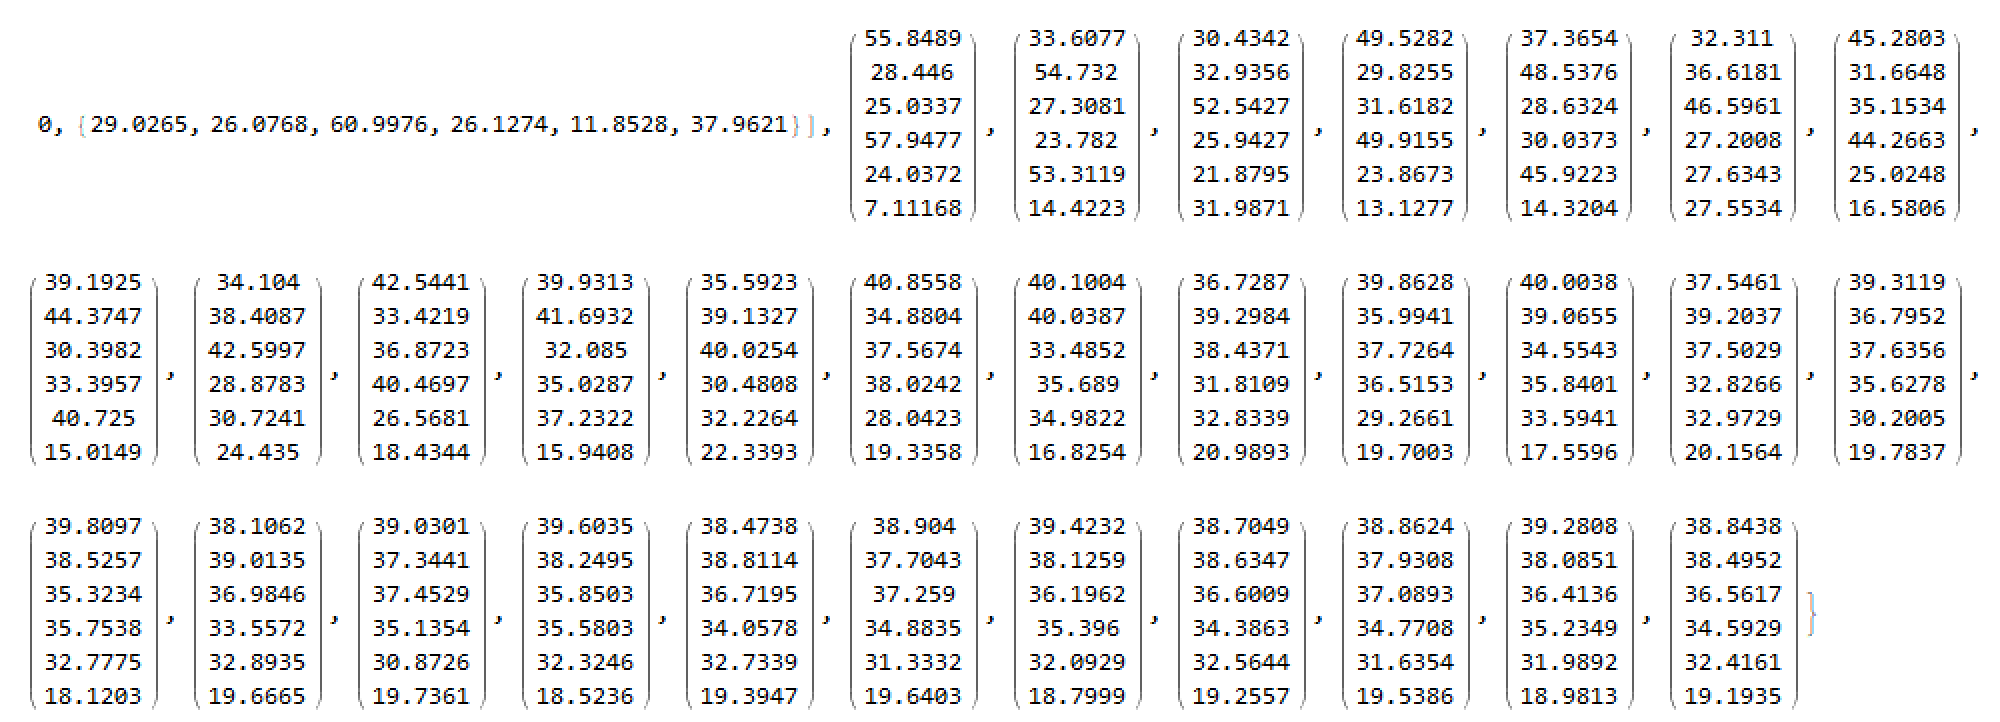
\includegraphics[width=\linewidth]{NewStartingPopulation.PNG}
  \caption{Showing the cycle based on the other eigenvectors}
\end{figure}

\end{document}